
\documentclass[tikz]{standalone}
\usepackage{graphicx}
\usepackage{lmodern}
\usepackage{amsmath, amssymb, amsfonts}
\usetikzlibrary{calc}
\newcommand{\R}{\mathcal{R}}

\begin{document}



%geometrically calculated surrogate
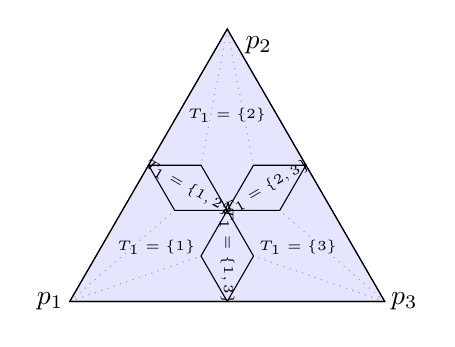
\begin{tikzpicture}
\draw[fill=blue, fill opacity = 0.1] (2,0) -- (-2,0) -- (0,3.46) -- cycle;
%label outcomes
\node at (-9/4, 0) {$p_1$};
\node at (2/5, 3.25) {$p_2$};
\node at (9/4, 0) {$p_3$};

%level sets
%kites
\draw (-2,0) --(0,0) -- (-1/3, 0.577) -- (0,2/1.73) -- (-2/3, 2/1.73) -- (-1, 1.73) -- cycle; 
\draw (2,0) -- (0,0) -- (1/3, 0.577) -- (0,2/1.73) -- (2/3, 2/1.73) --(1,1.73) -- cycle; 
\draw (0,3.46) --(-1, 1.73) -- (-1/3, 1.73) -- (0,2/1.73) -- (1/3, 1.73) --(1,1.73) -- cycle; 

%dashed lines
\draw[opacity=0.3, dotted] (-2,0) -- (-1/3, 0.577) ; 
\draw[opacity=0.3, dotted] (-2,0) -- (-2/3, 2/1.73) ; 
\draw[opacity=0.3, dotted] (0,3.46) -- (-1/3, 1.73) ; 
\draw[opacity=0.3, dotted] (0,3.46) -- (1/3, 1.73) ; 
\draw[opacity=0.3, dotted] (2,0) -- (1/3, 0.577) ; 
\draw[opacity=0.3, dotted] (2,0) -- (2/3, 2/1.73) ; 


%diamonds
%\draw (0,0) -- (-1/3, 0.577) -- (0,2/1.73) -- (1/3, 0.577) -- cycle; 
%\draw (-1, 1.73) -- (-2/3, 2/1.73) -- (0,2/1.73) -- (-1/3, 1.73) -- cycle; 
%\draw (1, 1.73) -- (2/3, 2/1.73) -- (0,2/1.73) -- (1/3, 1.73) -- cycle; 


%nodes
\node at (-.9, 1.73/2.5){\fontsize{3}{12}\selectfont  $T_1 = \{1\}$};
\node at (0, 3 * 1.73/2.2){\fontsize{3}{12}\selectfont  $T_1 = \{2\}$};
\node at (.9, 1.73/2.5){\fontsize{3}{12}\selectfont  $T_1 = \{3\}$};

\node[rotate=-30] at (-.5, 1.443){\fontsize{3}{12}\selectfont  $T_1 = \{1,2\}$};
\node[rotate=-90] at (0, 1.73/3){\fontsize{3}{12}\selectfont  $T_1 = \{1,3\}$};
\node[rotate=30] at (.5, 1.443){\fontsize{3}{12}\selectfont  $T_1 = \{2,3\}$};

%\node at (-2/3, 1/4){\fontsize{3}{12}\selectfont $(2,0,1)$};
%\node at (2/3, 1/4){\fontsize{3}{12}\selectfont $(1,0,2)$};
%\node at (-2/3, 0.577 * 1.4){\fontsize{3}{12}\selectfont $(1,0,0)$};
%\node at (2/3, 1.4*0.577){\fontsize{3}{12}\selectfont $(0,0,1)$};
%\node[rotate=52.5] at (-1.1, 2/1.73){\fontsize{3}{12}\selectfont $(2,1,0)$};
%\node[rotate=-52.5] at (1.1, 2/1.73){\fontsize{3}{12}\selectfont $(0,1,2)$};
%\node at (-1/2, 1.443){\fontsize{3}{12}\selectfont $(1,1,0)$};
%\node at (1/2, 1.443){\fontsize{3}{12}\selectfont $(0,1,1)$};
%\node at (0,1.73) {\fontsize{3}{12}\selectfont$(0,1,0)$};
%\node[rotate=-52.5] at (1/2, 1.73 + 1/2) {\fontsize{3}{12}\selectfont$(0,2,1)$};
%\node[rotate=52.5] at (-1/2, 1.73 + 1/2) {\fontsize{3}{12}\selectfont$(1,2,0)$};
\end{tikzpicture}


\end{document}
%%% Local Variables:
%%% mode: latex
%%% TeX-master: t
%%% End:
